\documentclass[12pt]{article}

\usepackage{fullpage}
\usepackage[cm-default]{fontspec}
\usepackage{xgreek}
\usepackage{float}
\usepackage{xunicode}
\usepackage{xltxtra}
\usepackage{algorithm}
\usepackage{algpseudocode}
\usepackage{amsmath}
\usepackage{mathtools}
\usepackage{unicode-math}
\usepackage{fontspec}
\usepackage{caption}
\usepackage{subcaption}
\usepackage{soul}

\setmainfont{CMU Serif}

\title{Ανάπτυξη Λογισμικού για Πληροφοριακά Συστήματα}
\author{Πανγιώτης Φωτόπουλος\\
  \texttt{sdi1300195@di.uoa.gr}
  \and Μάνος Πιτσικάλης\\
  \texttt{sdi1300143@di.uoa.gr}}
\date{}

\begin{document}

\maketitle


\section{Βασικές Δομές - Γενικά}
Για την αποθήκευση του γράφου χρησιμοποιούνται δύο ευρετήρια (index-buffer) ένα για τις εξερχόμενες ακμές και ένα για τις εισερχόμενες ακμές. Στις αναζητήσεις και όπου χρείαζονται λίστες,για την αποφυγή πολλών malloc, χρησιμοποιούνται λίστες υλοποιημένες με πίνακα ,οι οποιές και επαναχρησιμοποιούνται όταν χρειάστει. Δηλάδη γινέται μια φορά malloc, αν χρειαστεί γίνεται realloc, και με την λήξη της εκτέλεσης γίνεται η αποδέσμευση της μνήμης. Επιπλέον στις αναζητήσεις και όπου αλλού χρειάζεται δομή αποθηκεύσης επίσκεψης π.χ.(στην bidirectional-bfs δομή visited) χρησιμοποιείται πίνακας A ίσος με των αριθμό των στοιχείων με versioning, δηλαδή αν το στοιχείο x έχει επισκεφτεί οταν γίνεται αναζήτηση με version v τότε A[x]=v, αν καποιό στοιχείο y δεν έχει επισκεφτεί τότε θα ισχύει A[y]<v ,έτσι η αρχικοποιήση γίνεται μόνο μία φορά καί ο έλεγχος γίνεται σε O(1).
\section{Λεπτομέρειες υλοποίησης Part 1}
\section{Λεπτομέρειες υλοποίησης Part 2}
\section{Λεπτομέρειες υλοποίησης Part 3}
\section{Δοκιμές στην υλοποίηση}
\section{Μετρήσεις}
Σύγκριση Part1 Part2 Part3\\
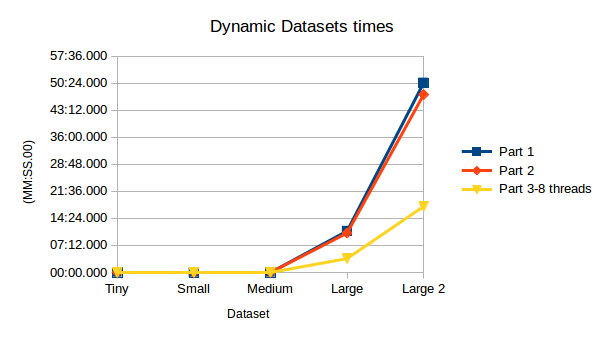
\includegraphics[scale=0.5]{DynamicDatasets_times.png}
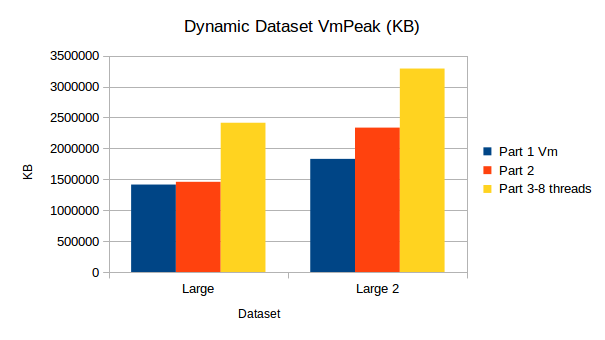
\includegraphics[scale=0.5]{DynamicDatasets_VmPeak.png}\\
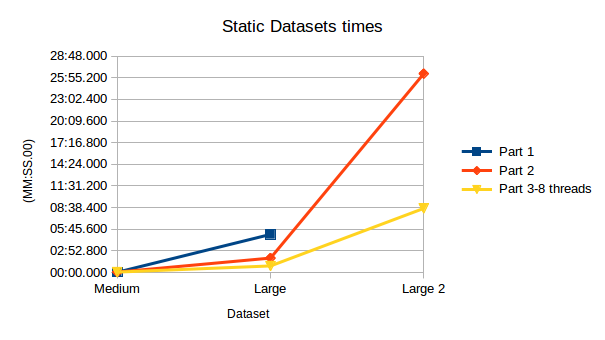
\includegraphics[scale=0.5]{StaticDatasets_times.png}
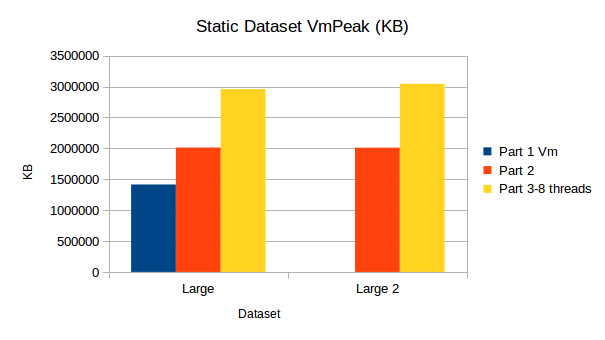
\includegraphics[scale=0.5]{StaticDatasets_VmPeak.png}\\
Σύγκριση Part3 αριθμός νημάτων\\
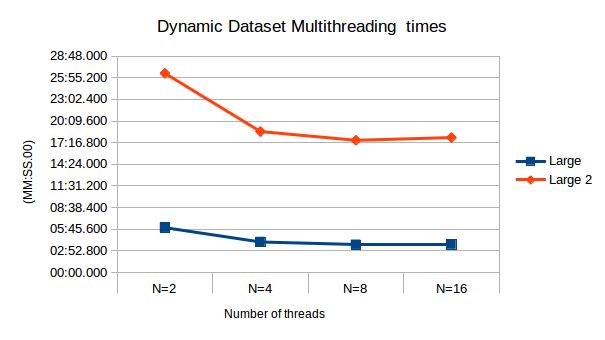
\includegraphics[scale=0.5]{DynamicDatasetMultithreading_times.png}
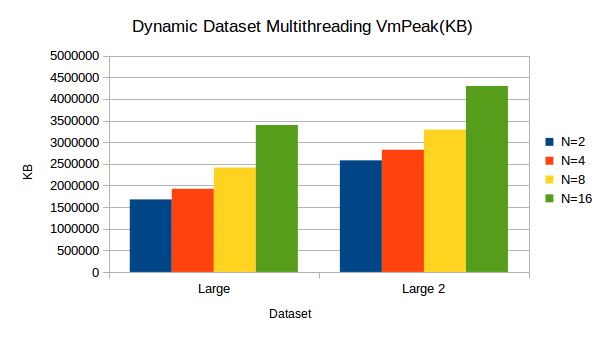
\includegraphics[scale=0.5]{DynamicDatasetMultithreading_VmPeak.png}\\
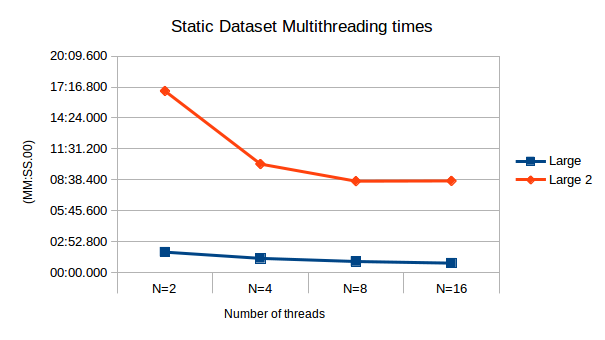
\includegraphics[scale=0.5]{DynamicStaticMultithreading_times.png}
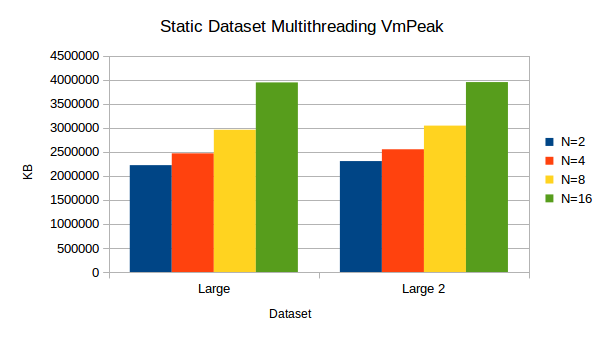
\includegraphics[scale=0.5]{DynamicStaticMultithreading_VmPeak.png}
\end{document}
